\documentclass[times, utf8, diplomski]{fer}

\usepackage{booktabs}
\usepackage{tikz}
\usepackage{indentfirst}
\usepackage{pgfplots}
\usepackage{graphicx}
\usepackage{caption}
\usepackage{subcaption}
\usepackage{graphicx}

\usetikzlibrary{matrix,calc}

\begin{document}

\thesisnumber{1382}
\title{Image Based Phylogenetic Classification}
\author{Vinko Kodžoman}

\maketitle

% Ispis stranice s napomenom o umetanju izvornika rada. Uklonite naredbu \izvornik ako želite izbaciti tu stranicu.
\izvornik

% Dodavanje zahvale ili prazne stranice. Ako ne želite dodati zahvalu, naredbu ostavite radi prazne stranice.
\zahvala{Thank you...}

\tableofcontents

\chapter{Introduction}
Since the dawn of time, people have tried to explain their surroundings. Life is all around us in many forms, and as such people have tried to categorize it by keen observation, both through its visual and genetic features. Today, it is organised into a taxonomic hierarchy of eight major taxonomic ranks. The number of known species on Earth is in the millions and climbing every year. Great numbers of species make it difficult to classify species based on images and requires domain knowledge. Therefore, an algorithm with the capability to classify species on the filed or from an image using only the image itself could provide great benefits for field researches.

Machine learning allows computers the ability to learn without being explicitly programmed \citep{samuel_studies_1959}. It, together with an incrase in avaiable quallity data (ImageNet, CIFAR -> dodati reference) has yielded great results in the area of deep learning - a class of machine learning algorithms. Deep learning algorithm's accuracy scales with the amount of data used by the algorithm (referenca), that together with the improvements in hardware - mainly general purpose graphic units (GPUs) - has yielded significant perfomance gains in the last couple of years. One of the most rapidly advancing filed of deep learning is image recognition (VGG16, Inception, Resnet -> reference) with new neural network architectures being developed almost at a yearly basis, the pefromance of deep neural networks on image recognition has achived results perviously tought 	impossible.

In this thesis I propose a solution for a scalable classification of species from images, based on convolution neural networks and recent modern deep learning techqniues.

\chapter{Research context}
To fully understand the depth of the image recognition using deep learning, we need a better understand of the underlying algorithms and methods in machine learning, as well as fundemental terms and concepts. In the next section, an introduction of basic terms is given, followed by a detailed explenation of fundemental machine learning algorithms.

\section{Definitions and notation}

\subsection{Image representation}
Matrix is a rectangular array of numberes. It is used because some numbers are naturally represented as matricies. Matrix $A$ with $m$ rows and $n$ columns often writtens as $m \times n$ has $m*n$ elements and is denoted as $A_{m,n}$. Elements are denoted as $a_{i,j}$ where $i$ and $j$ corespond to row and column number respectivly, as shown in \ref{eq_2d_matrix}. 

\begin{equation} \label{eq_2d_matrix}
A_{m,n} = 
 \begin{bmatrix}
  a_{1,1} & a_{1,2} & \cdots & a_{1,n} \\
  a_{2,1} & a_{2,2} & \cdots & a_{2,n} \\
  \vdots  & \vdots  & \ddots & \vdots  \\
  a_{m,1} & a_{m,2} & \cdots & a_{m,n} 
 \end{bmatrix}
\end{equation}


Each image is represented as a 3 dimensional matrix. One pixel in the image represent a single element in the matrix and as images have multiple channels (RGB) each channel is a 2 dimensional matrix. Image $I$ denoted as $I_{k,m,n}$ where $k\in[0,2]$ represent the channel - red, green or blue - and $m,n\in[0,255]$ represent the pixels in a particular channel as 2 dimensional matricies. Figure \ref{fig:image_matrix} shows a representation of an image as a 3 dimensional matrix where each pixel is denote as $I_{k,m,n}$.


\begin{figure}
\centering
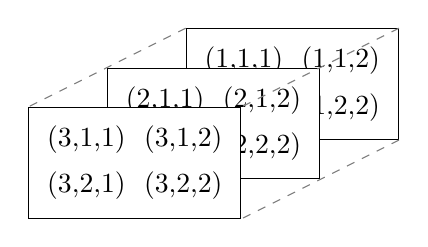
\begin{tikzpicture}
\def\xs{1} %shift in x direction
\def\ys{0.5} %shift in y direction
\def\nm{3} % number of 2d matrices in the 3d matrix
\foreach \x in {1,2,...,\nm}
{

\matrix [draw, % for the rectangle border
         fill=white, % so that it is not transparent
         ampersand replacement=\&] %see explanation
(mm\x)%give the matrix a name
at(-\x * \xs, -\x * \ys) %shift the matrix
{
    \node {(\x,1,1)}; \& \node {(\x,1,2)};\\
    \node {(\x,2,1)}; \& \node {(\x,2,2)};\\
};
}

\draw [dashed,gray](mm1.north west) -- (mm\nm.north west);
\draw [dashed,gray](mm1.north east) -- (mm\nm.north east);
\draw [dashed,gray](mm1.south east) -- (mm\nm.south east);
\end{tikzpicture}
\caption{RGB image with 4 pixels  represented as a 3 dimensional matrix}
\label{fig:image_matrix}
\end{figure}

\subsection{Gradient}
A gradient is a generalization of the derivative in multi-variable space and as such it is represented as a vector. Like the derivative, it represents the slope of the tanget of the graph of the function. Therefore, it points in the direction of the greatest rate of incrase of the function. Gradients are widely used in optimization theory as they allow the parameters to shift in a direction which will minimize or maximize a given function. In machine learning the function we want to minimize will be the loss function, which we will define in further chapters in more detail. Gradient of $f$ is denoted as $\nabla{f}$, where every component of $\nabla{f}$ is a partial derivavate of $f$, denoted as $\frac{\partial{f}}{\partial{x}}\mathbf{e}$. Notice that gradient components are vectors denoted as $\mathbf{e}$. Every vector is written as a bolded letter. The gradient for a $n$ dimensional space is defined in \ref{eq:gradient}.

\begin{equation} \label{eq:gradient}
    \nabla{f}= \frac{\partial{f}}{\partial{x_{1}}}\mathbf{e_1} + \hdots + 	   \frac{\partial{f}}{\partial{x_{n}}}\mathbf{e_n}
\end{equation}

\subsection{Activation functions}
Machine learning models use nonlinear functions to gain more capacity - expressiveness
. The most popular nonlinear functions are $sigmoid$, $tanh$, $relu$. All nonlinear functions have to have easy to compute gradients, as they are compunted on parameters in order to reduce loss as explained above. 
\begin{equation} \label{eq:sigmoid}
	sigmoid(x) = \frac{1}{1 + e^{-x}}
\end{equation}

\begin{equation} \label{eq:tanh}
	tanh(x) = \frac{1 - e^{-2x}}{1 + e^{-2}}
\end{equation}

\begin{equation} \label{eq:relu}
	relu(x) = max(0, x)
\end{equation}
The order of nonlinear functions is given in order of their discoveries. Today relu is used the most, since it solves the problem of vanishing gradiens for very deep neural networks, this does not apply to all network types. Reccurent neural networks (RNN) are a class of neural networks that often use $tanh$ as it is better suited for the particular reccurent architecture.

\begin{figure}
    \begin{subfigure}[b]{0.32\textwidth}
        \centering
        \resizebox{\linewidth}{!}{
            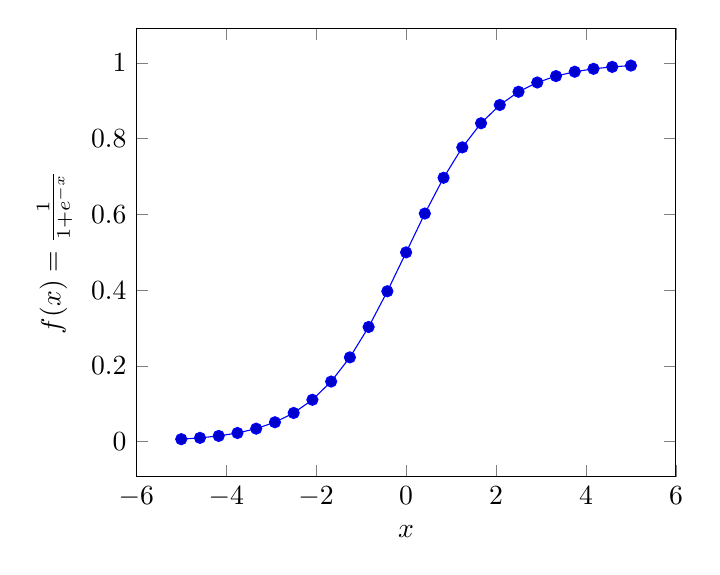
\begin{tikzpicture}
  			\begin{axis}[ 
	  			mark=none,
    			xlabel=$x$,
		    	ylabel={$f(x) = \frac{1}{1 + e^{-x}}$}
		    	] 
	   	 	\addplot {1 /(1 + e^-x)}; 
  			\end{axis}
            \end{tikzpicture}
        }
        \caption{$simgoid$}
        \label{fig:sigmoid}
    \end{subfigure}
    \begin{subfigure}[b]{0.32\textwidth}
    \centering
        \resizebox{\linewidth}{!}{
            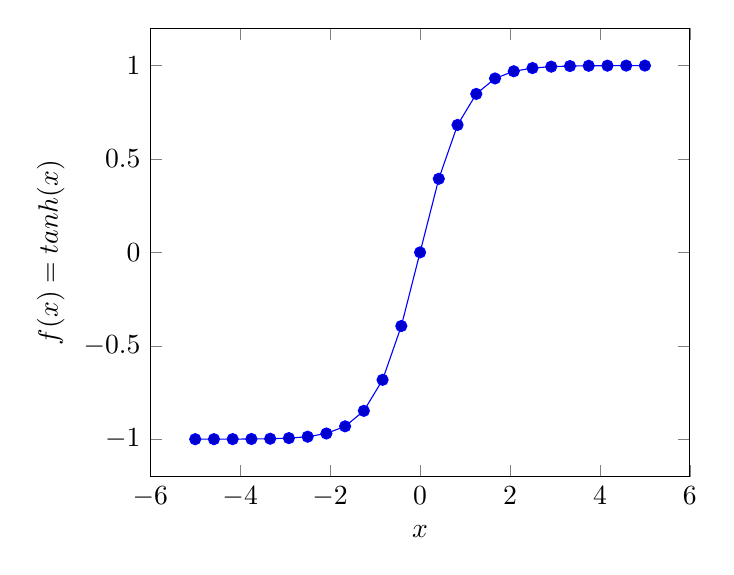
\begin{tikzpicture}
  			\begin{axis}[ 
	  			mark=none,
    			xlabel=$x$,
		    	ylabel={$f(x) = tanh(x)$}
		    	] 
	   	 	\addplot {tanh(x)}; 
  			\end{axis}
            \end{tikzpicture}
        }
        \caption{$tanh$}   
        \label{fig:tanh}
    \end{subfigure}
    \begin{subfigure}[b]{0.32\textwidth}
        \centering
        \resizebox{\linewidth}{!}{
            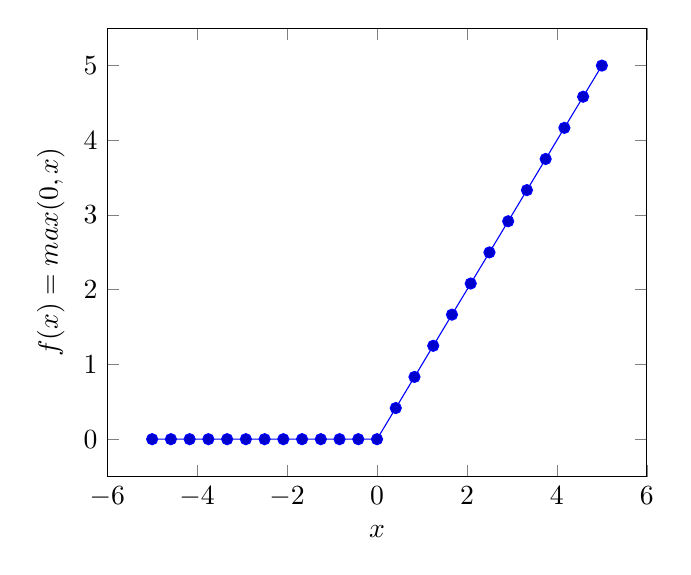
\begin{tikzpicture}
  			\begin{axis}[
  				mark=none,
    			xlabel=$x$,
		    	ylabel={$f(x) = max(0, x)$}
		    	] 
	   	 	\addplot {max(0,x)}; 
  			\end{axis}
            \end{tikzpicture}
        }
        \caption{$relu$}
        \label{fig:relu}
    \end{subfigure}
\caption{Nonliear activation functions} 
\label{fig:subfig1.a.4}
\end{figure}

\subsection{Metrics}
In order to compare different models a set of metrics is employed. Accuracy which gives the accuracy of a model, it is often used on balance datasets (\ref{eq:accuracy}). The problem with unbalanced datasets can be easily explained with a short example. Image having $2$ klasses $K=\{dog,cat\}$ and there are a total of $100$ images in the dataset, of which only $2$ are dogs. The model if optimized for accuracy might say the whole dataset is cats which will yeild an accuracy of $98\%$. To solve the previous problem, more metrics where introduced for the task of classification; precision (\ref{eq:precision}), recall (\ref{eq:recall}) and F1 score (\ref{eq:f1score}). Precision - positive predictive value - is defined as a fraction of retrived instances that are relevant. Recall - sensitivity - is a fraction of relevant instances that are retreived. In order to represent the perfromance of a model as a single variable F1 score was introduced, it represent a harmonic mean of accuracy and precision.
\begin{equation} \label{eq:accuracy}
	Accuracy = \frac{tp + tn}{tp + tn + fp + fn}
\end{equation}

\begin{equation} \label{eq:precision}
	Precision = \frac{tp}{tp + fp}
\end{equation}

\begin{equation} \label{eq:recall}
	Recall = \frac{tp}{tp + fn}
\end{equation}

\begin{equation} \label{eq:f1score}
	F1 score = 2 * \frac{precision * recall}{precision + recall}
\end{equation}


Classification results are often represented as a confusion matrix, also known as an error matrix.  It is a performance visualisation of a classification model - classifier. To build the classification matrix, conditions of the experiment must be labeled as positive and negative. Using the cats and dogs example from before and marking the cats and a positive and dogs as a negative class. Doing so creates a $2x2$ matrix of actual and predicted values as shown in table \ref{tb:confusion_matrix}.

\begin{table}
\centering
\caption{Confusion matrix}
\label{tb:confusion_matrix}
\begin{tabular}{|c|c|c|}
\hline 
 & \textbf{prediciton} positive & \textbf{prediction} negative \\ 
\hline 
\textbf{actual} positive & True Positive (TP) & False Positive (FP) \\ 
\hline 
\textbf{actual} negative & False Negative (FN) & True Negative (TN) \\ 
\hline 
\end{tabular}
\end{table}

\section{Machine learning}
What is,,..

Classification, regression, ....
\subsection{Supervised and unsupervised learning}
Supervised vs unsupervised.

\subsection{Models}
\subsection{Model selection}

\section{Deep learning}
GPUs

\subsection{Feedforward Neural Networks}
\subsection{Convolutional Neural Networks}
\subsection{Backpropagation}
\subsection{Vanishing Gradient}
\subsection{Batch Normalization}
\subsection{Data Augmentation}


\chapter{TaxNet}
Let's hope it is any good.
\section{Implementation}

\chapter{Dataset}
\subsection{ImageNet}

\chapter{Results}
Graphs graphs graphs...

\chapter{Conclusion}
Zaključak.

\bibliographystyle{fer}
\bibliography{master_thesis}


\begin{sazetak}
Sažetak na hrvatskom jeziku.

\kljucnerijeci{Ključne riječi, odvojene zarezima.}
\end{sazetak}

% TODO: Navedite naslov na engleskom jeziku.
\engtitle{Title}
\begin{abstract}
Abstract.

\keywords{Keywords.}
\end{abstract}

\end{document}